\documentclass[12pt,t]{beamer}
% \documentclass[t]{beamer}
\usepackage[utf8]{inputenc}
\usepackage[catalan]{babel}
\usepackage{verbatim}
\usepackage{hyperref}
\usepackage{amsfonts,amssymb,amsmath,amsthm, wasysym, multirow}
\usepackage{listings}
\usepackage[T1]{fontenc}        
\usepackage{pgf}
\usepackage{epsdice}
\usepackage{pgfpages}
\usepackage{tikz}
%\usetikzlibrary{arrows,shapes,plotmarks,backgrounds,trees,positioning}
%\usetikzlibrary{decorations.pathmorphing,calc,snakes}
%\usepackage{marvosym}
%
\usepackage{pgfpages}
\pgfpagesuselayout{4 on 1}[a4paper,border shrink=5mm,landscape]
\setbeamertemplate{footline}[frame number]
\usecolortheme{sidebartab}
\useinnertheme[shadow]{rounded}
% \useoutertheme[footline=empty,subsection=true,compress]{infolines}
% \useoutertheme[footline=empty,subsection=true,compress]{miniframes}
% \usefonttheme{serif}

\setbeamertemplate{caption}[numbered]
\setbeamertemplate{navigation symbols}{}


\newcommand{\red}[1]{\textcolor{red}{#1}}
\newcommand{\green}[1]{\textcolor{green}{#1}}
\newcommand{\blue}[1]{\textcolor{blue}{#1}}
\newcommand{\gray}[1]{\textcolor{gray}{#1}}
\renewcommand{\emph}[1]{{\color{red}#1}}

\setbeamertemplate{frametitle}
{\begin{centering}
\medskip
\color{blue}
\textbf{\insertframetitle}
\medskip
\end{centering}
}
\usecolortheme{rose}
\usecolortheme{dolphin}
\mode<presentation>


\newcommand{\CC}{\mathbb{C}}
\newcommand{\RR}{\mathbb{R}}
\newcommand{\ZZ}{\mathbb{Z}}
\newcommand{\NN}{\mathbb{N}}
\newcommand{\KK}{\mathbb{K}}
\newcommand{\MM}{\mathcal{M}}
%\newcommand{\dbinom}{\displaystyle\binom}

\newcommand{\limn}{{\displaystyle \lim_{n\to\infty}}}
\renewcommand{\leq}{\leqslant}
\renewcommand{\geq}{\geqslant}
\def\tendeix{{\displaystyle\mathop{\longrightarrow}_{\scriptscriptstyle
n\to\infty}}}

\newcommand{\matriu}[1]{\left(\begin{matrix} #1 \end{matrix}\right)}

% \newcommand{\qed}{\hbox{}\nobreak\hfill\vrule width 1.4mm height 1.4mm depth 0mm
%     \par \goodbreak \smallskip}
%
% %
\theoremstyle{plain}
\newtheorem{teorema}{Teorema}
\newtheorem{prop}{Proposició}
\newtheorem{cor}{Coro\l.lari}
\theoremstyle{definition}
\newtheorem{exemple}{Exemple}
\newtheorem{defin}{Definició}
\newtheorem{obs}{Observació}

\newcounter{seccions}
\newcommand{\seccio}[1]{\addtocounter{seccions}{1}
\medskip\par\noindent\emph{\theseccions.
#1}\smallskip\par }

\newcommand{\EM}{\Omega}
\newcommand{\PP}{\mathcal{P}}

\title[\red{Matemàtiques II}]{}
\author[]{}
\date{}



\begin{document}
\beamertemplatedotitem

\lstset{backgroundcolor=\color{green!50}}
\lstset{breaklines=true}
\lstset{basicstyle=\ttfamily}


\begin{frame}
\vfill
\begin{center}
\gray{\LARGE Regressió lineal}
\end{center}
\vfill
\end{frame}



\section{Regressió lineal simple}
\subsection{Regressió lineal}

\begin{frame}
\frametitle{Regressió lineal}

La taula següent dóna l'alçada mitjana (en cm) dels nins a determinades edats (en anys):
\begin{center}
\begin{tabular}{c|ccccccc}
\hline
edat & 1 & 3 & 5 & 7 & 9 & 11 & 13\\
\hline
alçada & 75 & 92 & 108 & 121 & 130 & 142 & 155\\
\hline
\end{tabular}
\end{center}
La segona setmana de Matemàtiques I calculàvem amb R la millor relació lineal
$$
\mbox{alçada}\approx b_0+b_1\cdot\mbox{edat}
$$ 
\end{frame}



\begin{frame}[fragile]
\frametitle{Regressió lineal}
\vspace*{-2ex}

\begin{verbatim}
> edat=c(1,3,5,7,9,11,13)
> alçada=c(75,92,108,121,130,142,155)
> plot(edat,alçada)
> abline(lm(alçada~edat))
\end{verbatim}
\vspace*{-4ex}

\begin{center}
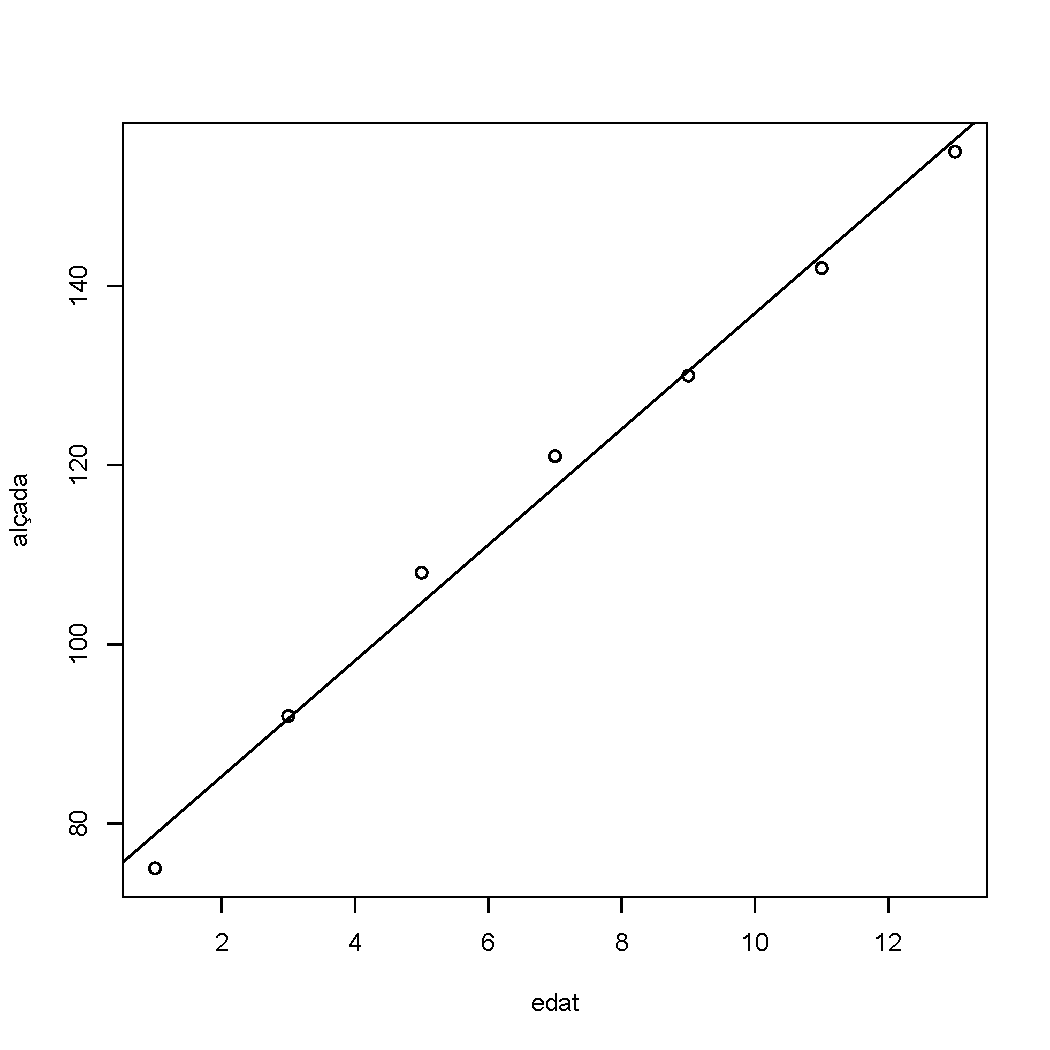
\includegraphics[width=0.7\linewidth]{ed-al2.pdf}
\end{center}
\end{frame}

\begin{frame}
\frametitle{Regressió lineal simple}
Tenim parelles d'observacions de dues variables $X,Y$:
$$
(x_i,y_i)_{i=1,2,\ldots,n}
$$
i volem estudiar com el valor de $Y$ depèn del de $X$:
\medskip

\begin{itemize}
\item La variable aleatòria $Y$ és la variable \emph{dependent} o \emph{de resposta}

\item La variable (no necessàriament aleatòria) $X$ és la variable \emph{de control},
\emph{independent} o \emph{de regressió}
\end{itemize}
\bigskip

Volem trobar la millor relació funcional que  expliqui la variable $Y$ conegudes les observacions de la
variable $X$. Per ara, cercam una \emph{relació lineal} que expliqui $Y$ en funció de $X$.
\end{frame}

\begin{frame}
\frametitle{Regressió lineal simple}

Suposam que 
$$
\mu_{Y|x}=\beta_0+\beta_1 x
$$
on $\mu_{Y|x}$ és el valor esperat de $Y$ quan $X$ val $x$, i $\beta_0$
(\emph{terme independent}) i $\beta_1$ (\emph{pendent}) són dos
paràmetres que volem estimar
\medskip

Amb una mostra $(x_i,y_i)_{i=1,2,\ldots,n}$, calcularem estimacions $b_0$ i $b_1$ de
$\beta_0$ i de $\beta_1$
\medskip

Això ens donarà la \emph{recta de regressió} per a la nostra mostra:
$$
\widehat{y}=b_0+b_1 x
$$
que donat un valor $x_0$ de $X$ ens estimarà el valor $\widehat{y}_0=b_0+b_1 x_0$ de $Y$ sobre el mateix individu
\end{frame}

\begin{frame}
\frametitle{Regressió lineal simple}

El model anterior el reescrivim com a
$$
Y|x=\beta_0+\beta_1 x+ E_x,
$$
on
\begin{itemize}
\item $Y|x$ és la variable aleatòria ``valor de $Y$ quan $X$ val $x$''
\medskip

\item $E_x$ és la variable aleatòria \emph{error} o \emph{residu}, dóna la diferència entre el valor de $Y$ i el valor ``mitjà'  $\beta_0+\beta_1 x$
\medskip

\item Com que suposam $\mu_{Y|x}=\beta_0+\beta_1 x$, suposam que $\mu_{E_x}=0$ per a cada $x$
\end{itemize}

\end{frame}

\subsection{Mínims quadrats}

\begin{frame}
\frametitle{Mínims quadrats}

Per a cada observació $(x_i,y_i)$, tendrem
$$
y_i=\beta_0+\beta_1 x_i+ \varepsilon_i\Rightarrow \varepsilon_i=y_i-(\beta_0+\beta_1 x_i)
$$
\smallskip

Diguem l'\emph{error quadràtic teòric} d'aquest model a
$$
\red{SS_\varepsilon}=\sum_{i=1}^n \varepsilon_i^2=\sum_{i=1}^n (y_i-\beta_0-\beta_1 x_i)^2
$$
A la \emph{regressió lineal per mínims quadrats}, els estimadors $b_0$ i $b_1$ de $\beta_0$ i $\beta_1$ que cercam són els valors de ``les incògnites''  $\beta_0$ i $\beta_1$ que minimitzen aquest  $SS_\varepsilon$.
\end{frame}

\begin{frame}
\frametitle{Mínims quadrats}
El mínim $(b_0,b_1)$ de
$$
SS_\varepsilon=\sum_{i=1}^n (y_i-\beta_0-\beta_1 x_i)^2
$$
anu\l.la les derivades respecte de $\beta_0$ i $\beta_1$.
\medskip

Derivem:
$$
\begin{array}{ll}
\dfrac{\partial SS_\varepsilon}{\partial \beta_0}=&-2\sum\limits_{i=1}^n (y_i -\beta_0-\beta_1 x_i)\\[2ex]
\dfrac{\partial SS_\varepsilon}{\partial \beta_1}=&-2\sum\limits_{i=1}^n (y_i -\beta_0-\beta_1 x_i) x_i 
\end{array}
$$
\end{frame}

\begin{frame}
\frametitle{Mínims quadrats}
El $(b_0,b_1)$ que cercam satisfà
$$
\begin{array}{l}
2\sum\limits_{i=1}^n (y_i -b_0-b_1 x_i)=0\\[2ex]
2\sum\limits_{i=1}^n (y_i -b_0-b_1 x_i) x_i =0
\end{array}
$$
Reescrivim:
$$
\begin{array}{rl}
n b_0 + \Big(\sum\limits_{i=1}^n x_i\Big) b_1 & =\sum\limits_{i=1}^n y_i\\[1ex]
\Big(\sum\limits_{i=1}^n x_i\Big) b_0 + \Big(\sum\limits_{i=1}^n x_i^2\Big) b_1 &=\sum\limits_{i=1}^n x_iy_i
\end{array}
$$
\end{frame}

\begin{frame}
\frametitle{Mínims quadrats}
Les solucions són
$$
\begin{array}{rl}
b_1& \displaystyle=\frac{n \sum\limits_{i=1}^n x_i y_i-\sum\limits_{i=1}^n x_i\sum\limits_{i=1}^n y_i} {n\sum\limits_{i=1}^n
x_i^2-(\sum\limits_{i=1}^n x_i)^2}\\[6ex]
b_0& \displaystyle=\frac{\sum\limits_{i=1}^n y_i -b_1 \sum\limits_{i=1}^n x_i}{n}
\end{array}
$$
i  donen el mínim de $SS_\varepsilon$
\end{frame}

\begin{frame}
\frametitle{Mínims quadrats}
Considerem les mitjanes
$$
\overline{x}=\frac{1}{n}\sum\limits_{i=1}^n x_i,
\quad \overline{y}=\frac{1}{n} \sum\limits_{i=1}^n y_i
$$
i les variàncies i covariància 
$$
\begin{array}{rl}
s_x^2 &\displaystyle =\frac{1}{n}\sum_{i=1}^n (x_i-\overline{x})^2 =\frac{1}{n}\Big(\sum_{i=1}^n x_i^2\Big) -\overline{x}^2\\[2ex]
s_y^2 &\displaystyle =\frac{1}{n}\sum_{i=1}^n (y_i-\overline{y})^2 =\frac{1}{n}\Big(\sum_{i=1}^n y_i^2\Big) -\overline{y}^2\\[2ex]
s_{xy} &\displaystyle =\frac{1}{n}\sum_{i=1}^n (x_i-\overline{x}) (y_i-\overline{y}) =\frac{1}{n}\Big(\sum_{i=1}^n x_i y_i\Big)-\overline{x}\cdot\overline{y}
\end{array}
$$
\end{frame}

\begin{frame}
\frametitle{Mínims quadrats}
Els valors de $b_0$ i $b_1$ trobats abans es poden reescriure de la forma següent:

\begin{teorema}
Els estimadors $b_0$ i $b_1$ per mínims quadrats de $\beta_0$ i $\beta_1$ són
$$
b_1 =\frac{s_{xy}}{s_x^2},\quad b_0 = \overline{y}-b_1 \overline{x}.
$$
\end{teorema}
Escriurem
$$
\widehat{y}=b_0+b_1x
$$
Direm a $\widehat{y}$ el \emph{valor estimat} de $Y$ quan $X=x$
\medskip

Per a cada dada $(x_i,y_i)$, en direm l'\emph{error} a 
$$
\red{e_i}=y_i-\widehat{y}_i={y}_i-b_0-b_1x_i
$$
\end{frame}

\begin{frame}[fragile]
\frametitle{Exemple 1}
Volíem calcular la recta de regressió per mínims quadrats de
\begin{center}
\begin{tabular}{c|ccccccc}
\hline
edat ($x$) & 1 & 3 & 5 & 7 & 9 & 11 & 13\\
\hline
alçada ($y$) & 75 & 92 & 108 & 121 & 130 & 142 & 155\\
\hline
\end{tabular}
\end{center}
\begin{verbatim}
> x=c(1,3,5,7,9,11,13)
> y=c(75,92,108,121,130,142,155)
> x.b=mean(x)
> y.b=mean(y)
> s2.x=var(x)*6/7
> s2.y=var(y)*6/7
> s.xy=cov(x,y)*6/7
> round(c(x.b,y.b,s2.x,s2.y,s.xy),3)
[1]   7.000 117.571  16.000 674.531 103.429
\end{verbatim}
\end{frame}

\begin{frame}[fragile]
\frametitle{Exemple 1}
\vspace*{-2ex}

\begin{center}
\begin{tabular}{cccccccc}
$\overline{x}$ &  $\overline{y}$ & $s_x^2$ & $s_y^2$ & $s_{xy}$\\ \hline
7.000 & 117.571 & 16 & 674.531 & 103.429
\end{tabular}
\end{center}
$$
\begin{array}{l}
\displaystyle b_1 =\frac{s_{xy}}{s_x^2}=\frac{103.429}{16}=6.4643\\[2ex]
\displaystyle b_0 = \overline{y}-b_1 \overline{x} =117.571-6.4643\cdot 7=72.3209
\end{array}
$$
Obtenim
$$
\widehat{y}=72.3209+6.4643x
$$
\medskip

\begin{verbatim}
> lm(y~x)$coefficients
(Intercept)           x 
  72.321429    6.464286 
\end{verbatim}
\end{frame}

\begin{frame}[fragile]
\frametitle{Alerta!}

Els càlculs involucrats en la regressió lineal són molt poc robusts: els arrodoniments
poden influir molt en el resultat final
\bigskip

A la Wikipedia (\url{http://en.wikipedia.org/wiki/Simple_linear_regression}) hi trobareu un exemple detallat d'una regressió de pes en funció d'alçada. Calculada en metres dóna:
$$
\widehat{y}=61.272x-39.062
$$
Si es passen les alçades a polzades, s'arrodoneixen, es calcula la recta de regressió, i es torna a passar  el resultat a metres, dóna
$$
\widehat{y}=61.675x-39.746
$$




\end{frame}



\begin{frame}
\frametitle{Exemple 2}
En un experiment on es volia estudiar l'associació entre consum de sal i pressió arterial, a alguns individus se'ls assignà aleatòriament una quantitat diària constant de sal en la seva dieta, i al cap d'un mes se'ls mesurà la tensió mitjana. Alguns resultats varen ser els següents
\begin{center}
\begin{tabular}{cc}
$X$ (sal, en g) 	& $Y$ (Pressió, en mm de Hg)\\ \hline
1.8 &	100\\
2.2 &	98\\
3.5 &	110\\
4.0 &	110\\
4.3 &	112\\
5.0 &	120\\
\end{tabular}
\end{center}
Trobau la recta de regressió lineal per mínims quadrats de $Y$ en funció de $X$

\end{frame}

\begin{frame}
\frametitle{Exemple 2}

\begin{center}
\begin{tabular}{ccccc}
$\overline{x}$ &  $\overline{y}$ & $s_x^2$ & $s_y^2$ & $s_{xy}$\\ \hline
3.467 & 108.333 & 1.2856 &55.2222 & 8.1444
\end{tabular}
\end{center}
\bigskip

$$
\begin{array}{l}
\displaystyle b_1 =\vphantom{\frac{s_{xy}}{s_x^2}}\hphantom{\overline{y}-b_1 \overline{x} = 86.371}\\[2ex]
\displaystyle b_0 =\hphantom{\overline{y}-b_1 \overline{x} = 86.371}
\end{array}
$$
\bigskip

Obtenim la recta
$$
\widehat{y}= \hphantom{86.371+6.335x}
$$

\end{frame}


\begin{frame}
\frametitle{Propietats}

\begin{itemize}
\item La recta de regressió passa pel vector mitjà
$(\overline{x},\overline{y})$:
$$
b_0+b_1 \overline{x}=\overline{y}
$$

\item La mitjana dels valors estimats és igual a la mitjana dels
observats:
$$
\red{\overline{\widehat{y}}=}\frac{1}{n}\sum_{i=1}^n\widehat{y}_i
=\frac{1}{n}\sum_{i=1}^n(b_0+b_1x_i)=
b_0+b_1 \overline{x}=\red{\overline{y}}
$$

\item Els errors $(e_i)_{i=1,\ldots,n}$ tenen mitjana 0:
$$
\hspace*{-0.7cm}\red{\overline{e}
=}\frac{1}{n}\sum_{i=1}^n e_i
=\frac{1}{n}\sum_{i=1}^n (y_i-b_0-b_1x)
=\frac{1}{n}\sum_{i=1}^n (y_i-\widehat{y}_i)
=\red{0}
$$
\end{itemize}
\end{frame}



\begin{frame}
\frametitle{Propietats}
Direm \emph{suma de quadrats dels errors} a
$$
\red{SS_E}=\sum_{i=1}^{n} e^2_i
$$
\medskip

Els errors $(e_i)_{i=1,\ldots,n}$ tenen variància
$$
\red{s_e^2=}\frac{1}{n}\Big(\sum_{i=1}^{n}
e^2_i\Big)-\overline{e}^2=\red{\frac{SS_E}{n}}
$$

\end{frame}


\begin{frame}
\frametitle{Propietats}

\begin{teorema}
Si les variables aleatòries error $E_{x_i}$ tenen totes mitjana 0 i la mateixa variància $\sigma^2_E$ i, dues a dues, tenen covariància 0, aleshores

\begin{itemize}
\item $b_0$ i $b_1$ són estimadors lineals no esbiaixats òptims (més eficients) de $\beta_0$ i $\beta_1$
\medskip

\item Un estimador no esbiaixat de $\sigma_E^2$ és
$$
S^2=\frac{SS_E}{n-2}
$$
\end{itemize}
\end{teorema}
\end{frame}



\begin{frame}
\frametitle{Propietats}

\begin{teorema}
Si \emph{a més} les variables aleatòries error $E_{x_i}$ són normals, aleshores
 $b_0$ i $b_1$ són els estimadors màxim versemblants de $\beta_0$ i $\beta_1$ (i no esbiaixats)
 \end{teorema}
\end{frame}





\begin{frame}[fragile]
\frametitle{Exemple 1}
Si suposam que al nostre exemple d'edats i alçades els errors tenen la mateixa variància i són incorrelats, podem estimar aquesta variància:
\begin{verbatim}
> x=c(1,3,5,7,9,11,13)
> y=c(75,92,108,121,130,142,155)
> y.cap=72.321+6.464*x
> errors=y-y.cap
> SSE=sum(errors^2)
> S2=SSE/(length(x)-2)
> S2
[1] 8.314296
\end{verbatim}
Tenim que $S^2=8.3143$, i estimam que $\sigma_E^2$ val això
\end{frame}

\begin{frame}[fragile]
\frametitle{Exemple 2}
Si suposam que al nostre exemple de sal i tensió arterial els errors  tenen la mateixa variància i són incorrelats, podem estimar aquesta variància:
\begin{verbatim}
> sal=c(1.8,2.2,3.5,4,4.3,5)
> ten=c(100,98,110,110,112,120)
> ten.cap=86.371+6.335*sal
> errors.ten=ten-ten.cap
> SSE=sum(errors.ten^2)
> S2=SSE/(length(sal)-2)
> S2
[1] 5.436475
\end{verbatim}
Tenim que $S^2=5.4365$, i estimam que $\sigma_E^2$ val això
\end{frame}





\begin{frame}
\frametitle{Això és tot?}
Hem estimat els coeficients $\beta_0$ i $\beta_1$ i la variable $Y|x$, per a cada $x$,  al model
$$
\mu_{Y|x}=\beta_0+\beta_1 x
$$
però ens pot interessar més:
\medskip

\begin{itemize}
\item Com és de significativa l'estimació obtinguda?
\medskip

\item Error estàndard d'aquests estimadors
\medskip

\item Intervals de confiança 
\end{itemize}
\end{frame}




\begin{frame}[fragile]
\frametitle{Amb R obtenim molt més\ldots}
\footnotesize \begin{verbatim}
> summary(lm(alçada~edat))
...
Coefficients:
            Estimate Std. Error t value Pr(>|t|)    
(Intercept)  72.3214     2.1966   32.92 4.86e-07 ***
edat          6.4643     0.2725   23.73 2.48e-06 ***
---
Signif. codes:  0 ‘***’ 0.001 ‘**’ 0.01 ‘*’ 0.05
   ‘.’ 0.1 ‘ ’ 1 

Residual standard error: 2.883 on 5 degrees of freedom
Multiple R-squared: 0.9912,	Adjusted R-squared: 0.9894 
F-statistic: 562.9 on 1 and 5 DF,  p-value: 2.477e-06 
\end{verbatim}
\end{frame}


\subsection{Coeficient de determinació}
\begin{frame}[fragile]
\frametitle{Com és de significativa la regressió?}

Entenem que la recta $\widehat{y}=b_0+b_1x$ és una bona aproximació de $y$ com a funció lineal de $x$ quan molta part de la variabilitat de $y$ l'explica aquesta recta.
\bigskip

Es quantifica amb el \emph{coeficient de determinació $R^2$}
\begin{verbatim}
> summary(lm(alçada~edat))$r.squared
[1] 0.9911957
\end{verbatim}

\end{frame}

\begin{frame}
\frametitle{Sumes de quadrats}
Siguin:
\begin{itemize}
\item $\red{SS_T} =\sum\limits_{i=1}^n(y_i-\overline{y})^2$: suma de quadrats de totals
$$
SS_T=n\cdot s_y^2
$$

\item $\red{SS_R}=\sum\limits_{i=1}^n(\widehat{y}_i-\overline{y})^2$: suma de quadrats de la regressió 
$$
SS_R=n\cdot s_{\widehat{y}}^2
$$

\item $\red{SS_E}=\sum\limits_{i=1}^n(y_i-\widehat{y}_i)^2$: suma de quadrats dels errors
$$
SS_E=n\cdot s_e^2
$$
\end{itemize}

\end{frame}

\begin{frame}
\frametitle{Sumes de quadrats}

\begin{teorema}
En una regressió lineal pel mètode de mínims quadrats, es té que
$$
SS_T=SS_R+SS_E
$$
o equivalentment,
$$
s^2_y=s^2_{\widehat{y}}+s^2_e
$$
\end{teorema}

\end{frame}
%
%\begin{frame}[fragile]
%\frametitle{Exemple 1}
%\vspace*{-2ex}
%
%\begin{verbatim}
%> x=c(1,3,5,7,9,11,13)
%> y=c(75,92,108,121,130,142,155)
%> y.cap=72.321+6.464*seq(1,13,2)
%> errors=y-y.cap
%> SST=sum((y-mean(y))^2)
%> SSR=sum((y.cap-mean(y))^2)
%> SSE=sum((y-y.cap)^2)
%> c(SST,SSR,SSE)
%[1] 4721.71429 4679.72919   41.57148
%> SSR+SSE
%[1] 4721.301
%\end{verbatim}
%\end{frame}
%
%
%\begin{frame}[fragile]
%\frametitle{Exemple 1}
%\vspace*{-2ex}
%
%
%\begin{verbatim}
%> x=c(1,3,5,7,9,11,13)
%> y=c(75,92,108,121,130,142,155)
%> lm(y~x)$coefficients
%(Intercept)           x 
%  72.321429    6.464286 
%> y.cap=lm(y~x)$coefficients[1]+lm(y~x)$coefficients[2]*seq(1,13,2)
%> errors=y-y.cap
%> SST=sum((y-mean(y))^2)
%> SSR=sum((y.cap-mean(y))^2)
%> SSE=sum(errors^2)
%> c(SST,SSR,SSE)
%[1] 4721.71429 4680.14286   41.57143
%> SSR+SSE
%[1] 4721.714
%\end{verbatim}
%\end{frame}
%

\begin{frame}
\frametitle{El coeficient de determinació $R^2$}
El \emph{coeficient de determinació} d'una regressió lineal és
$$
\red{R^2}=\frac{SS_R}{SS_T}=\frac{s_{\widehat{y}}^2}{s_y^2}
$$
Per tant, $R^2$ és la fracció de la variabilitat de $y$ que queda explicada per la variabilitat de $\widehat{y}$
\bigskip


Si la regressió lineal és per mínims quadrats,
$$
R^2=\frac{SS_T-SS_E}{SS_T}=1-\frac{SS_E}{SS_T}=1-\frac{s_e^2}{s_y^2}
$$
\end{frame}


\begin{frame}
\frametitle{El coeficient de determinació $R^2$}
A més, \emph{$R^2=r_{xy}^2$}, el coeficient de correlació al quadrat
$$
\begin{array}{rl}
R^2 & \displaystyle =\frac{SS_R}{SS_T}=\frac{\sum\limits_{i=1}^n(b_1x_i+b_0-\overline{y})^2}{s_y^2}\\[2ex] 
& \displaystyle =\frac{\sum\limits_{i=1}^n(\frac{s_{xy}}{s_x^2}x_i-\frac{s_{xy}}{s_x^2}\overline{x})^2}{s_y^2}\\[2ex] 
& \displaystyle =\frac{\frac{s_{xy}^2}{s_x^4}\sum\limits_{i=1}^n(x_i-\overline{x})^2}{s_y^2}\\[2ex] & \displaystyle =\frac{s_{xy}^2}{s_x^4}\cdot \frac{s_x^2}{s_y^2}=\frac{s_{xy}^2}{s_x^2\cdot s_y^2}=r_{xy}^2
\end{array}
$$
\end{frame}

%
%\begin{frame}
%\frametitle{El coeficient de determinació $R^2$}
%A més:
%
%\begin{itemize}
%\item Un estimador no esbiaixat de $\sigma_E^2$ (la variància de la variable aleatòria Error $E$) és
%$$
%S^2=\frac{SS_E}{n-2}
%$$
%\end{itemize}
%\end{frame}

\begin{frame}[fragile]
\frametitle{Exemple 1}
\vspace*{-2ex}

\begin{verbatim}
> x=c(1,3,5,7,9,11,13)
> y=c(75,92,108,121,130,142,155)
> y.cap=72.321+6.464*x
> SST=sum((y-mean(y))^2)
> SSR=sum((y.cap-mean(y))^2)
> SSE=sum((y-y.cap)^2)
> round(c(SST,SSR,SSE),3)
[1] 4721.714 4679.729  41.571
\end{verbatim}
$$
R^2=\frac{4679.729}{4721.714}=0.9912
$$
\begin{verbatim}
> cor(x,y)^2
[1] 0.9911957
\end{verbatim}
\end{frame}

\begin{frame}[fragile]
\frametitle{Exemple 2}
\vspace*{-3ex}

\small \begin{verbatim}
> sal=c(1.8,2.2,3.5,4,4.3,5)
> ten=c(100,98,110,110,112,120)
> ten.cap=86.371+6.335*sal
> SST=sum((ten-mean(ten))^2)
> SSR=sum((ten.cap-mean(ten))^2)
> SSE=sum((ten-ten.cap)^2)
> round(c(SST,SSR,SSE),3)
[1] 331.333 309.553  21.746
\end{verbatim}
$$
R^2=
$$
\end{frame}


\subsection{Intervals de confiança}

\begin{frame}
\frametitle{Supòsits del model}

Suposam d'ara endavant que \emph{cada $E_{x_i}$ segueix una distribució normal amb mitjana $\mu_{E_{x_i}}=0$, la mateixa variància $\sigma_E^2$, i $\sigma(E_{x_i},E_{x_j})=0$ per a cada parella $i,j$}
\bigskip

Si només tenim molt pocs $y$ per a cada $x$, això no es pot contrastar, però implica que els $(e_i)_{i=1,\ldots,n}$ provenen d'una $N(0,\sigma_E^2)$, amb $\sigma_E^2$ estimada per $S^2$, i això sí que ho podem contrastar
\end{frame}

\begin{frame}[fragile]
\frametitle{Exemple 1}
A l'exemple de les alçades i les edats
\begin{verbatim}
> x=c(1,3,5,7,9,11,13)
> y=c(75,92,108,121,130,142,155)
> y.cap=72.321+6.464*x
> errors=y-y.cap
> SSE=sum(errors^2)
> S2=SSE/5
> ks.test(errors,"pnorm",0,S2)
      One-sample Kolmogorov-Smirnov test
data:  errors 
D = 0.3399, p-value = 0.3182
alternative hypothesis: two-sided 
\end{verbatim}
\end{frame}

\begin{frame}[fragile]
\frametitle{Exemple 2}
A l'exemple de la sal i la tensió
\begin{verbatim}
> sal=c(1.8,2.2,3.5,4,4.3,5)
> ten=c(100,98,110,110,112,120)
> ten.cap=86.371+6.335*sal
> errors=ten-ten.cap
> SSE=sum(errors^2)
> S2=SSE/4
> ks.test(errors,"pnorm",0,S2)
      One-sample Kolmogorov-Smirnov test
data:  errors 
D = 0.3411, p-value = 0.3965
alternative hypothesis: two-sided 
\end{verbatim}
\end{frame}

\begin{frame}
\frametitle{Intervals de confiança}
\begin{teorema}
Sota aquestes hipòtesis,
\begin{itemize}
\item Els errors estàndard dels estimadors $b_1$ i $b_0$ són, respectivament,
$$
\frac{\sigma_E}{s_x\sqrt{n}}\quad\mbox{ i }\quad \frac{\sigma_E\sqrt{s_x^2+\overline{x}^2}}{s_x\sqrt{n}}
$$
\end{itemize}
\end{teorema}
\medskip

En aquests errors estàndard (i tots els que segueixen), estimam $\sigma_E$ per mitjà de $S=\sqrt{S^2}$

\end{frame}


\begin{frame}
\frametitle{Intervals de confiança}
\begin{teorema}
Sota aquestes hipòtesis,
\begin{itemize}
\item Les fraccions
$$
\frac{b_1-\beta_1}{\frac{S}{s_x\sqrt{n}}}\quad\mbox{ i }\quad
\frac{b_0-\beta_0}{\frac{S\sqrt{s_x^2+\overline{x}^2}}{s_x\sqrt{n}}}
$$
segueixen lleis $t$ de Student amb $n-2$ graus de llibertat.
\end{itemize}
\end{teorema}

\end{frame}


\begin{frame}
\frametitle{Intervals de confiança}
\vspace*{-2ex}

Per tant, sota aquestes hipòtesis,
\begin{itemize}
\item Un interval de confiança del $(1-\alpha)\cdot 100\%$ per $\beta_1$ és
$$
\left] b_1-t_{n-2,1-\frac{\alpha}{2}} \frac{S}{s_x\sqrt{n}}, b_1+t_{n-2,1-\frac{\alpha}{2}} \frac{S}{s_x\sqrt{n}}\right[
$$
Ho escriurem
$$
\beta_1=b_1\pm t_{n-2,1-\frac{\alpha}{2}} \frac{S}{s_x\sqrt{n}}
$$





\item Un interval de confiança del $(1-\alpha)\cdot 100\%$ per $\beta_0$ és
$$
\beta_0=b_0\pm t_{n-2,1-\frac{\alpha}{2}}\frac{S\sqrt{s_x^2+\overline{x}^2}}{s_x\sqrt{n}}
$$
\end{itemize}

\end{frame}

\begin{frame}
\frametitle{Exemple 1}
\vspace*{-2ex}

A l'exemple de les alçades en funció de l'edat, havíem obtingut la recta
$$
\widehat{y}=72.321+6.464x
$$
i $\overline{x}=7$, $s_x^2=16$, $n=7$, $S^2=8.314$
\medskip

Un interval de confiança al 95\% per $\beta_1$ és
$$
\begin{array}{l}
\displaystyle \beta_1=b_1\pm t_{n-2,1-\frac{\alpha}{2}} \frac{S}{s_x\sqrt{n}}
\\[2ex]
\displaystyle\hphantom{\beta_1} =6.464\pm t_{5,0.975} \frac{\sqrt{8.314}}{4\sqrt{7}}\\[2ex]
\hphantom{\beta_1} =
6.464\pm 2.5706 \cdot 0.2724=6.464\pm  0.7
\end{array}
$$
És l'interval $]5.764,7.164[$
\end{frame}

\begin{frame}
\frametitle{Exemple 1}
\vspace*{-2ex}

A l'exemple de les alçades en funció de l'edat, havíem obtingut la recta
$$
\widehat{y}=72.321+6.464x
$$
i $\overline{x}=7$, $s_x^2=16$, $n=7$, $S^2=8.314$
\medskip

Un interval de confiança al 95\% per $\beta_0$ és
$$
\begin{array}{l}
\displaystyle \beta_0=b_0\pm t_{n-2,1-\frac{\alpha}{2}}\frac{S\sqrt{s_x^2+\overline{x}^2}}{s_x\sqrt{n}}
\\[2ex]
\displaystyle\hphantom{\beta_0}=72.321\pm t_{5,0.975} \frac{\sqrt{8.314}\cdot\sqrt{16+7^2}}{4\sqrt{7}}\\[2ex]
\hphantom{\beta_0} =
72.321\pm 2.5706 \cdot 2.1966=72.321\pm 5.647
\end{array}
$$
És l'interval $]66.674,77.968[$

\end{frame}






\begin{frame}[fragile]
\frametitle{Exemple 1}
\vspace*{-2ex}

Obtenim
\begin{itemize}
\item Interval del 95\% per a $\beta_1$: $]5.764,7.164[$
\medskip

\item Interval del 95\% per a $\beta_0$: $]66.674,77.968[$
\end{itemize}
\begin{verbatim}
> confint(lm(y~x),level=0.95)
                2.5 %    97.5 %
(Intercept) 66.674769 77.968088
x            5.763904  7.164668
\end{verbatim}

\end{frame}



\begin{frame}
\frametitle{Exemple 2}


A l'exemple de la tensió en funció de la sal, havíem obtingut la recta
$$
\widehat{y}=86.371+6.335x
$$
i $\overline{x}=3.467$, $s_x^2=1.2856$, $n=6$, $S^2=5.4365$, $t_{4,0.975}=2.7764$
\medskip

L'interval de confiança al 95\% per $\beta_1$ és

\end{frame}

\begin{frame}
\frametitle{Exemple 2}
\vspace*{-2ex}

A l'exemple de la tensió en funció de la sal, havíem obtingut la recta
$$
\widehat{y}=86.371+6.335x
$$
i $\overline{x}=3.467$, $s_x^2=1.2856$, $n=6$, $S^2=5.4365$, $t_{4,0.975}=2.7764$
\medskip

L'interval de confiança al 95\% per $\beta_0$ és

\end{frame}


\begin{frame}[fragile]
\frametitle{Exemple 2}
\vspace*{-2ex}

Obtenim
\begin{itemize}
\item Interval del 95\% per a $\beta_1$:  $]4.004,8.666[$
\medskip

\item Interval del 95\% per a $\beta_0$:   $]77.869, 94.873[$
\end{itemize}
\begin{verbatim}
> confint(lm(ten~sal),level=0.95)
                2.5 %    97.5 %
(Intercept) 77.869064 94.872509
sal          4.004434  8.666266
\end{verbatim}

\end{frame}



\begin{frame}
\frametitle{Intervals de confiança}
\begin{teorema}
Sota aquestes hipòtesis, i si $x_0$ és un possible valor de $X$
\begin{itemize}
\item L'error estàndard de $\widehat{y}_0$ com a estimador de $\mu_{Y|x_0}$ és
$$
\sigma_E\sqrt{\frac{1}{n}+\frac{(x_0-\overline{x})^2}{ns^2_x}}
$$

\item La fracció
$$
\frac{\widehat{y}_0-\mu_{Y/x_0}}{S\sqrt{\frac{1}{n}+\frac{(x_0-\overline{x})^2}{n
s^2_x}}}$$
segueix una llei $t$ de Student amb $n-2$ graus de llibertat.
\end{itemize}
\end{teorema}
\end{frame}


\begin{frame}
\frametitle{Intervals de confiança}
\begin{teorema}
Sota aquestes hipòtesis, i si $x_0$ és un possible valor de $X$
\begin{itemize}
\item L'error estàndard de $\widehat{y}_0$ com a estimador de $y_0$ és
$$
\sigma_E\sqrt{1+\frac{1}{n}+\frac{(x_0-\overline{x})^2}{ns^2_x}}
$$

\item La fracció
$$
\frac{\widehat{y}_0-y_0}{S\sqrt{1+\frac{1}{n}+\frac{(x_0-\overline{x})^2}{n
s^2_x}}}
$$
segueix una llei $t$ de Student amb $n-2$ graus de llibertat.
\end{itemize}
\end{teorema}
\end{frame}





\begin{frame}
\frametitle{Intervals de confiança}
Per tant, sota aquestes hipòtesis,
\begin{itemize}
\item Un interval de confiança del $(1-\alpha)\cdot 100\%$ per $\mu_{Y/x_0}$ és
$$
\mu_{Y/x_0}=\widehat{y}_0\pm t_{n-2,1-\frac{\alpha}{2}} S\sqrt{\frac{1}{n}+\frac{(x_0-\overline{x})^2}{n
s^2_x}}
$$

\item Un interval de confiança del $(1-\alpha)\cdot 100\%$ per $y_0$ és
$$
y_0=\widehat{y}_0\pm t_{n-2,1-\frac{\alpha}{2}} S\sqrt{1+\frac{1}{n}+\frac{(x_0-\overline{x})^2}{n
s^2_x}}
$$
\end{itemize}

\end{frame}



\begin{frame}
\frametitle{Exemple 1}
\vspace*{-2ex}

A l'exemple de les alçades en funció de l'edat, havíem obtingut la recta
$$
\widehat{y}=72.321+6.464x
$$
i $\overline{x}=7$, $s_x^2=16$, $n=7$, $S^2=8.314$
\medskip

Suposem que volem estimar l'alçada $y_0$ d'un nin de $x_0=10$ anys  
$$
\widehat{y}_0=72.321+6.464\cdot 10=136.961
$$

Interval de confiança al 95\% per aquest valor? Interval de confiança al 95\% per al valor esperat?
\end{frame}



\begin{frame}
\frametitle{Exemple 1}
\vspace*{-2ex}


Un interval de confiança al 95\% per $y_0$ és
$$
\begin{array}{l}
\displaystyle
y_0=\widehat{y}_0\pm t_{n-2,1-\frac{\alpha}{2}} S\sqrt{1+\frac{1}{n}+\frac{(x_0-\overline{x})^2}{ns^2_x}}
\\[2ex]
\displaystyle\hphantom{y_0}=136.961\pm t_{5,0.975} \sqrt{8.314}\cdot\sqrt{1+\frac{1}{7}+\frac{(10-7)^2}{7\cdot 16 }}\\[2ex]
\hphantom{y_0} =
136.961\pm 2.5706 \cdot  3.189=136.961\pm  8.198
\end{array}
$$
És l'interval $]128.8,145.2[$

\end{frame}


\begin{frame}
\frametitle{Exemple 1}
\vspace*{-2ex}


Un interval de confiança al 95\% per $\mu_{Y|x_0}$ és
$$
\begin{array}{l}
\displaystyle
\mu_{Y|x_0}=\widehat{y}_0\pm t_{n-2,1-\frac{\alpha}{2}} S\sqrt{\frac{1}{n}+\frac{(x_0-\overline{x})^2}{ns^2_x}}
\\[2ex]
\displaystyle\hphantom{y_0}=136.961\pm t_{5,0.975} \sqrt{8.314}\cdot\sqrt{\frac{1}{7}+\frac{(10-7)^2}{7\cdot 16 }}\\[2ex]
\hphantom{y_0} =
136.961\pm 2.5706 \cdot  1.362=136.961\pm  3.501
\end{array}
$$
És l'interval $]133.5, 140.5[$

\end{frame}


\begin{frame}[fragile]
\frametitle{Exemple 1}
\vspace*{-2ex}

\begin{verbatim}
> regressio=lm(y~x)
> newdata=data.frame(x=10)
> predict.lm(lm(y~x),newdata,
  interval="prediction",level=0.95)
       fit      lwr     upr
1 136.9643 128.7665 145.162
> predict(lm(y~x),newdata,
  interval="confidence",level=0.95)
       fit      lwr      upr
1 136.9643 133.4624 140.4662
\end{verbatim}



\end{frame}

\begin{frame}
\frametitle{Té sentit una regressió lineal?}

Si $\beta_1=0$,  el model de regressió lineal no té sentit:
$$
Y=\beta_0+E
$$
i les variacions en els valors de $Y$ són totes degudes a l'error.
\medskip

El contrast
$$
\left\{\begin{array}{l}
H_0:\beta_1=0\\
H_1:\beta_1 \neq 0
\end{array}
\right.
$$
el podem realitzar amb l'interval de confiança per a $\beta_1$: si 0 no hi pertany, 
rebutjam la hipòtesi nu\l.la
\end{frame}


\begin{frame}
\frametitle{Exemples}
\vspace*{-2ex}

Hem obtingut:
\begin{itemize}
\item A l'exemple 1, un interval del 95\% per a $\beta_1$ és $]5.764,7.164[$
\medskip

\item A l'exemple 2, un interval del 95\% per a $\beta_1$:  $]4.004,8.666[$
\end{itemize}
\medskip

Als dos casos concloem que $\beta_1\neq 0$ i que per tant tenia sentit fer la regressió lineal
\end{frame}

\begin{frame}[fragile]
\frametitle{Amb R}
{\footnotesize \begin{verbatim}
> summary(lm(alçada~edat))
...
Coefficients:
            Estimate Std. Error t value Pr(>|t|)    
(Intercept)  72.3214     2.1966   32.92 4.86e-07 ***
edat          6.4643     0.2725   23.73 2.48e-06 ***
---
Signif. codes:  0 ‘***’ 0.001 ‘**’ 0.01 ‘*’ 0.05
   ‘.’ 0.1 ‘ ’ 1 
...
\end{verbatim}
}

Els \red{\texttt{t value}} són els dels contrastos amb $H_0:$ ``coeficient $=0$'', i els p-valors són els d'aquests
 contrastos. Podem rebutjar que $\beta_1=0$ (i que $\beta_0=0$)

\end{frame}

%\subsection{ANOVA}
%\begin{frame}
%\frametitle{ANOVA en la  regressió lineal}
%
%En el context de la regressió lineal, usarem ANOVA per contrastar si les mitjanes
%$$
%\left\{\begin{array}{l}
%H_0:\mu_{Y|x_1}=\ldots=\mu_{Y|x_n}\\
%H_1:\mbox{no és veritat que\ldots}
%\end{array}
%\right.
%$$
%Si aquestes mitjanes són iguals, no depenen de $x$ i per tant $\beta_1=0$ i el model de regressió lineal no té sentit: les variacions en els valors de $Y$ són totes degudes a l'error.
%\medskip
%
%Per tant, el significat d'aquest contrast és
%$$
%\left\{\begin{array}{l}
%H_0:\beta_1=0\\
%H_1:\beta_1 \neq 0
%\end{array}
%\right.
%$$
%i el model tendrà sentit si rebutjam la hipòtesi nu\l.la
%\end{frame}
%
%
%\begin{frame}
%\frametitle{ANOVA en la regressió lineal}
%
%Calculam la taula:
%\medskip
%
%\begin{center}
%\footnotesize \begin{tabular}{|c|c|c|c|c|c|}\hline
%Font de & Graus de & Suma de & Quadrats & $F$ & p-valor\\
%variació & llibertat &  quadrats & mitjans      &  & \\\hline
%Regressió & 1 & $SS_R$  & $SS_R$ & $SS_R/S^2$ &  p-valor\\
%Error & $n-2$ & $SS_E$  & $S^2$ & &\\
%\hline Total & $n-1$ & $SS_T$  & & &\\\hline
%\end{tabular}
%\end{center}
%\medskip
%
%Sota les hipòtesis usuals,
%$$
%F=\frac{SS_R}{S^2}
%$$
%segueix una distribució $F$ de Fisher amb 1 i $n-2$ graus de llibertat, i si és prou gran rebutjam la hipòtesi nu\l.la, per tant el p-valor és
%$$
%P(F_{1,n-2}\geq F)
%$$
%
%\end{frame}
%
%\begin{frame}
%\frametitle{Exemple 1}
%
%\begin{center}
%\footnotesize \begin{tabular}{|c|c|c|c|c|c|}\hline
%Font de & Graus de & Suma de & Quadrats & $F$ & p-valor\\
%variació & llibertat &  quadrats & mitjans      &  & \\\hline
%Regressió & 1 & $4679.723$  & $4679.723$ & $562.8$ &  0\\
%Error & 5 & $41.571$  & $8.314$ & &\\
%\hline Total &6 &  $4721.714$ & & &\\\hline
%\end{tabular}
%\end{center}
%\medskip
%
%El p-valor és 0, rebutjam la hipòtesi nu\l.la, el model lineal té sentit (a més, ja havíem obtingut $R^2\approx 0.99$ amb $b_1\neq 0$)
%\end{frame}
%
%
%
%\begin{frame}[fragile]
%\frametitle{Codi R}
%\footnotesize
%\begin{verbatim}
%> summary(aov(lm(y~x)))
%            Df Sum Sq Mean Sq F value   Pr(>F)    
%x            1   4680    4680   562.9 2.48e-06 ***
%Residuals    5     42       8                     
%---
%Signif. codes:  0 ‘***’ 0.001 ‘**’ 0.01 ‘*’ 0.05
%  ‘.’ 0.1 ‘ ’ 1 
%\end{verbatim}
%\end{frame}
%
%
%
%\begin{frame}[fragile]
%\frametitle{Codi R}
%\footnotesize
%\begin{verbatim}
%> summary(lm(y~x))
%...
%Residuals:
%      1       2       3       4       5       6       7 
%-3.7857  0.2857  3.3571  3.4286 -0.5000 -1.4286 -1.3571 
%
%Coefficients:
%            Estimate Std. Error t value Pr(>|t|)    
%(Intercept)  72.3214     2.1966   32.92 4.86e-07 ***
%x             6.4643     0.2725   23.73 2.48e-06 ***
%---
%Signif. codes:  0‘***’0.001‘**’0.01‘*’0.05‘.’0.1‘ ’1 
%
%Residual standard error: 2.883 on 5 degrees of freedom
%Multiple R-squared: 0.9912,	Adjusted R-squared: 0.9894 
%F-statistic: 562.9 on 1 and 5 DF,  p-value: 2.477e-06 
%\end{verbatim}
%\end{frame}


\section{Regressió lineal múltiple}
\subsection{Regressió lineal}

\begin{frame}
\frametitle{Regressió lineal múltiple}

Tenim ara $k$ variables (no necessàriament aleatòries) independents $X_1,\ldots, X_k$ i una
variable depenent $Y$.
\medskip

Suposam el model
$$
\mu_{Y|x_1,\ldots,x_k}= \beta_0+\beta_1 x_1+\cdots+\beta_k x_k.
$$
Els paràmetres $\beta_i$ són desconeguts i els estimam  a partir d'una mostra:
$$
(x_{i1},x_{i2},\ldots,x_{ik},y_i)_{i=1,\ldots,n}
$$
amb $n>k$ (el nombre d'observacions ha de ser més gran que el nombre de variables)
\medskip

Escriurem $\underline{x}_i=(x_{i1},x_{i2},\ldots,x_{ik})$
\end{frame}

\begin{frame}
\frametitle{Regressió lineal múltiple}
\vspace*{-2ex}

Traduïm aquest model en
$$
Y|x_1,\ldots,x_k=\beta_0+\beta_1 x_{1}+\cdots+\beta_{k} x_k+E_{x_1,\ldots,x_k}
$$
on
\begin{itemize}
\item $Y|x_1,\ldots,x_k$ és la v.a. que dóna el valor de $Y$ quan cada $X_i=x_i$
\medskip

\item $E_{x_1,\ldots,x_k}$ són les v.a. error, o residuals, i representen l'error aleatori del model associat a
$(x_1,\ldots,x_k)$
\end{itemize}

A partir d'una mostra
$$
(\underline{x}_{i},y_i)_{i=1,2,\ldots,n}
$$
obtendrem estimacions $b_0,b_1,\ldots,b_k$ dels paràmetres $\beta_0,\beta_1,\ldots,\beta_k$
\end{frame}


\begin{frame}
\frametitle{Regressió lineal múltiple}
Diguem
$$
\begin{array}{l}
\widehat{y}_i=b_0+b_1 x_{i 1}+\cdots+b_{k} x_{i k}\\
y_i=b_0+b_1 x_{i 1}+\cdots+b_{k} x_{i k}+e_i
\end{array}
$$
Aleshores
\begin{itemize}
\item $\widehat{y}_i$ és el valor predit de $y_i$ a partir de $\underline{x}_{i}$ i els estimadors $b_0,b_1,\ldots,b_k$ dels paràmetres
\medskip

\item $e_i$ estima l'error $E_{\underline{x}_{i}}$
\medskip

\item $e_i=y_i-\widehat{y}_i$
\end{itemize}
\end{frame}

\begin{frame}
\frametitle{Regressió lineal múltiple}
Escrivim-ho en forma matricial. Diguem
$$
\mathbf{y}=
\left(
\begin{array}{l}
y_1\\ y_2\\ \vdots\\ y_n
\end{array}
\right),\ \mathbf{b}=\left(
\begin{array}{l}
b_0\\ b_1 \\ \vdots\\b_k
\end{array}
\right),\ \mathbf{\widehat{y}}=\left(
\begin{array}{l}
\widehat{y}_1\\ \widehat{y}_2\\ \vdots\\\widehat{y}_n
\end{array}
\right),\ \mathbf{e}=\left(
\begin{array}{l}
e_1\\ e_2\\ \vdots\\ e_n
\end{array}
\right)
$$
\medskip

$$
\mathbf{X}=\left(
\begin{array}{lllll}
1&x_{11}&x_{12}&\ldots&x_{1k}\\
1&x_{21}&x_{22}&\ldots&x_{2k}\\
\vdots&\vdots&\vdots&\ddots&\vdots\\
1&x_{n1}&x_{n2}&\ldots&x_{nk}
\end{array}
\right)$$
\end{frame}


\begin{frame}[fragile]
\frametitle{Introducció}
Les equacions
$$
\begin{array}{l}
\widehat{y}_i=b_0+b_1 x_{i 1}+\cdots+b_{k} x_{i k}\\
y_i=b_0+b_1 x_{i 1}+\cdots+b_{k} x_{i k}+e_i
\end{array}
$$
corresponen a
$$
\begin{array}{l}
\mathbf{\widehat{y}} = \mathbf{X}\mathbf{b} \\
\mathbf{y}=   \mathbf{X}\mathbf{b}+\mathbf{e}\\
\end{array}
$$
\end{frame}

\subsection{Mínims quadrats}
\begin{frame}
\frametitle{Mètode dels mínims quadrats}

Definim l'\emph{error quadràtic} \red{$SS_E$} com:
$$
\begin{array}{rl}
\red{SS_E}=&\sum\limits_{i=1}^n
e^2_i=\sum\limits_{i=1}^n (y_i-\widehat{y}_i)^2 \\
=&\sum\limits_{i=1}^n (y_i-b_0-b_1 x_{i 1}-\cdots -b_{k} x_{ik})^2.
\end{array}
$$

Els estimadors de $\beta_0,\beta_1,\ldots, \beta_k$ pel mètode de mínims quadrats seran els
valors $b_0,b_1,\ldots, b_k$ que minimitzin $SS_E$
\end{frame}

\begin{frame}
\frametitle{Mètode dels mínims quadrats}

Per calcular-los, calculam les derivades parcials de $SS_E$ respecte de cada $b_i$, les igualam a 0, les resolem, i comprovam que la solució $(b_0,\ldots,b_k)$ trobada dóna un mínim\ldots
\medskip

\begin{teorema}
Els estimadors per mínims quadrats de $\beta_0,\beta_1,\ldots,\beta_k$ a partir de la mostra 
$(\underline{x}_{i},y_i)_{i=1,2,\ldots,n}$ són donats per l'equació següent:
$$
\mathbf{b}=\left(\mathbf{X}^t\cdot \mathbf{X}
\right)^{-1}\cdot \left(\mathbf{X}^t \cdot \mathbf{y}\right).
$$
\end{teorema}
\end{frame}

\begin{frame}
\frametitle{Exemple 3}

Es postula que l'alçada d'un nin nounat ($y$) té
una relació  lineal amb la seva edat en dies ($x_1$), la seva alçada en néixer en
cm ($x_2$), el seu pes en kg en néixer ($x_3$) i l'augment en tant per cent del seu pes actual respecte del seu pes en néixer ($x_4$). 
\medskip

El model és
$$
\mu_{Y|x_1,x_2,x_3,x_4}=\beta_0+\beta_1x_1+\beta_2x_2+\beta_3x_3+\beta_4x_4
$$
\medskip

En una mostra de $n=9$
nins, els resultats varen ser els de la taula següent:
\end{frame}

\begin{frame}
\frametitle{Exemple 3}

\begin{center}\begin{tabular}{|c|c|c|c|c|}\hline
$y$ & $x_1$ & $x_2$ & $x_3$ & $x_4$\\\hline
57.5&78&48.2&2.75&29.5\\ 52.8&69&45.5&2.15&26.3\\
61.3&77&46.3&4.41&32.2\\ 67&88&49&5.52&36.5\\ 53.5&67&43&3.21&27.2\\
62.7&80&48&4.32&27.7\\ 56.2&74&48&2.31&28.3\\ 68.5&94&53&4.3&30.3\\
69.2&102&58&3.71&28.7\\\hline\end{tabular}\end{center}

\end{frame}
\begin{frame}
\frametitle{Exemple 3}

La matriu $\mathbf{X}$ és:
$$
\mathbf{X}=\left(
\begin{array}{ccccc}
1&78&48.2&2.75&29.5\\
1&69&45.5&2.15&26.3\\
1&77&46.3&4.41&32.2\\
1&88&49&5.52&36.5\\
1&67&43&3.21&27.2\\
1&80&48&4.32&27.7\\
1&74&48&2.31&28.3\\
1&94&53&4.3&30.3\\
1&102&58&3.71&28.7
\end{array}
\right)
$$
\end{frame}

\begin{frame}
\frametitle{Exemple 3}
El vector $\mathbf{y}$ és:
$$
\mathbf{y}=\left(
\begin{array}{c}
57.5\\ 52.8\\ 61.3\\ 67\\ 53.5\\ 62.7\\ 56.2\\ 68.5\\ 69.2
\end{array}
\right)
$$
\end{frame}

\begin{frame}[fragile]
\frametitle{Exemple 3}
\vspace*{-2ex}

\small 
\begin{verbatim}
> X=
 matrix(c(1,78,48.2,2.75,29.5,1,69,45.5,2.15,26.3,
 1,77,46.3,4.41,32.2,1,88,49,5.52,36.5,
 1,67,43,3.21,27.2,1,80,48,4.32,27.7,
 1,74,48,2.31,28.3,1,94,53,4.3,30.3,
 1,102,58,3.71,28.7),nrow=9,byrow=TRUE)
> y=cbind(c(57.5,52.8,61.3,67,53.5,62.7,56.2,68.5,
  69.2))
\end{verbatim}
\end{frame}

\begin{frame}[fragile]
\frametitle{Exemple 3}
\vspace*{-2ex}

\small
\begin{verbatim}
> t(X)%*%X
       [,1]     [,2]      [,3]      [,4]      [,5]
[1,]   9.00   729.00   439.000   32.6800   266.700
[2,] 729.00 60123.00 35947.200 2702.4100 21715.300
[3,] 439.00 35947.20 21568.180 1604.3880 13026.010
[4,]  32.68  2702.41  1604.388  128.6602   990.268
[5,] 266.70 21715.30 13026.010  990.2680  7980.830
> t(X)%*%y
          [,1]
[1,]   548.700
[2,] 45001.000
[3,] 26946.890
[4,]  2035.521
[5,] 16348.290
\end{verbatim}
\end{frame}


\begin{frame}
\frametitle{Exemple 3}
El producte $\mathbf{X}^t\mathbf{X}$ és:
$$
\left(
\begin{array}{ccccc}
9& 729& 439& 32.68 & 266.7 \\
729& 60123& 35947.2& 2702.41& 21715.3\\
439& 35947.2& 21568.18& 1604.388& 13026.01\\
66.07 & 6108.19 & 3541.008& 128.66& 1948.561\\
266.7& 21715.3&13026.01& 990.27& 7980.83
\end{array}
\right)
$$
El producte $\mathbf{X}^t\mathbf{y}$ és
$$
\mathbf{X}^t\mathbf{y} = \left(
\begin{array}{c}
548.7\\ 45001\\ 26946.89\\ 2035.52\\ 16348.29
\end{array}
\right)
$$
\end{frame}

\begin{frame}
\frametitle{Exemple 3}
El vector d'estimadors dels coeficients $\beta_0,\beta_1,\ldots,\beta_4$ és
{\small $$
\begin{array}{l}
\mathbf{b}=\left(
\begin{array}{ccccc}
9& 729& 439& 32.68 & 266.7 \\
729& 60123& 35947.2& 2702.41& 21715.3\\
439& 35947.2& 21568.18& 1604.388& 13026.01\\
66.07 & 6108.19 & 3541.008& 128.66& 1948.561\\
266.7& 21715.3&13026.01& 990.27& 7980.83
\end{array}
\right)^{-1}\\
\hphantom{\mathbf{b}=}\ \cdot 
\left(
\begin{array}{c}
548.7\\ 45001\\ 26946.89\\ 2035.52\\ 16348.29
\end{array}
\right)
\end{array}
$$
}
\end{frame}

\begin{frame}[fragile]
\frametitle{Exemple 3}
\begin{verbatim}
> round(solve(t(X)%*%X)%*%(t(X)%*%y),4)
        [,1]
[1,]  7.1475
[2,]  0.1001
[3,]  0.7264
[4,]  3.0758
[5,] -0.0300
\end{verbatim}

\end{frame}

\begin{frame}
\frametitle{Exemple 3}
Obtenim
$$
\mathbf{b}=\left(
\begin{array}{l}
7.1475 \\ 0.1001 \\ 0.7264 \\ 3.0758\\ -0.03
\end{array}
\right)
$$
\medskip

La funció lineal de regressió cercada és:
$$
\widehat{y}=7.1475 + 0.1001 x_1+0.7264 x_2 +3.0758 x_3-0.03 x_4.
$$
\end{frame}

\begin{frame}[fragile]
\frametitle{Exemple 3}
\small
\begin{verbatim}
> Xd=X[,c(2:5)]
> lm(y~Xd)
Call:
lm(formula = y ~ Xd)
Coefficients:
(Intercept)      Xd1      Xd2      Xd3       Xd4  
    7.14753  0.10009  0.72642  3.07584  -0.03004  
\end{verbatim}
\end{frame}


\begin{frame}
\frametitle{Propietats}

\begin{itemize}
\item La recta de regressió passa pel vector mitjà
$(\overline{x}_1,\overline{x}_2,\ldots,\overline{x}_k,\overline{y})$:
$$
\overline{y}=b_0+b_1 \overline{x}_1+\cdots+b_1 \overline{x}_k
$$

\item La mitjana dels valors estimats és igual a la mitjana dels
observats:
$$
\overline{\widehat{y}}=\overline{y}
$$

\item Els errors $(e_i)_{i=1,\ldots,n}$ tenen mitjana 0 i variància
$$
s_e^2=\frac{SS_E}{n}
$$

\end{itemize}

\end{frame}








\subsection{Coeficient de determinació}
\begin{frame}
\frametitle{Sumes de quadrats}
Siguin
\begin{itemize}
\item $\red{SS_T}=\sum_{i=1}^n (y_i-\overline{y})^2$: suma de quadrats de totals.
$$
SS_T=n\cdot s_y^2
$$

\item $\red{SS_R}=\sum_{i=1}^n(\widehat{y}_i-\overline{y})^2$: suma de quadrats de la regressió.
$$
SS_R=n\cdot s_{\widehat{y}}^2
$$

\item $\red{SS_E}=\sum_{i=1}^n (y_i-\widehat{y}_i)^2$: suma de quadrats dels errors
$$
SS_E=n\cdot s_{e}^2
$$
\end{itemize}
\medskip

Si la regressió és per mínims quadrats,
$$
SS_T=SS_R+SS_E\mbox{ o, equivalentment, }
s^2_y=s^2_{\widehat{y}}+s^2_y
$$
\end{frame}


\begin{frame}
\frametitle{Coeficient de determinació}

El \emph{coeficient de determinació} d'una regressió lineal és
$$
\red{R^2}=\frac{SS_R}{SS_T}=\frac{s^2_{\widehat{y}}}{s^2_y}
$$
Representa la fracció de la variabilitat de $y$ que és explicada
per la variabilitat del model de regressió lineal
\medskip

El \emph{coeficient de correlació múltiple} de  $y$ respecte de $x_1,\ldots, x_k$ és
$$
R=\sqrt{R^2}
$$
\end{frame}


\begin{frame}
\frametitle{Coeficient de determinació}
\vspace*{-2ex}

$R^2$ tendeix a créixer amb $k$, encara que afegim variables redundants
\medskip

Per tenir-ho en compte, en lloc d'emprar
$$
R^2=\frac{SS_R}{SS_T}=\frac{SS_T-SS_E}{SS_T}
$$
s'empra el \emph{coeficient de determinació ajustat}
$$
\red{R^2_{adj}}=\frac{MS_T-MS_E}{MS_T}
$$
on 
$$
MS_T=\frac{SS_T}{n-1}, MS_E=\frac{SS_E}{n-k-1}
$$
Queda
$$
R^2_{adj}=1-(1-R^2)\frac{n-1}{n-k-1}
$$
\end{frame}

\begin{frame}[fragile]
\frametitle{Exemple 3}
\vspace*{-2ex}

Coeficients de determinació del nostre exemple
\begin{verbatim}
> # X i y ja definits
> b=solve(t(X)%*%X)%*%(t(X)%*%y)
> y.cap=X%*%b
> SS.T=sum((y-mean(y))^2)
> SS.R=sum((y.cap-mean(y))^2)
> SS.E=sum((y.cap-y)^2)
> round(c(SS.T,SS.R,SS.E),3)
[1] 321.240 318.274   2.966
\end{verbatim}
{\small $$
\begin{array}{l}
\displaystyle R^2=\frac{SS_R}{SS_T}=\frac{318.274}{321.24}=0.991\\[2ex]
\displaystyle R^2_{adj}=1-(1-R^2)\Big(\frac{9-1}{9-4-1}\Big)=0.982
\end{array}$$

}
\end{frame}

\begin{frame}[fragile]
\frametitle{Exemple 3}
\vspace*{-2ex}

\footnotesize \begin{verbatim}
> Xd=X[,c(2:5)]
> summary(lm(y~Xd))
...

Residual standard error: 0.861 on 4 degrees of freedom
Multiple R-squared: 0.9908,	Adjusted R-squared: 0.9815 
F-statistic: 107.3 on 4 and 4 DF,  p-value: 0.0002541 
> summary(lm(y~Xd))$r.squared
[1] 0.9907683
> summary(lm(y~Xd))$adj.r.squared
[1] 0.9815367
\end{verbatim}
\end{frame}

\begin{frame}[fragile]
\frametitle{Comparació de models}
Sovint ens interessarà comparar dos models lineals per a una mateixa variable depenent (per exemple, si afegim o llevam una variable, millora el model?)
\medskip

Aquesta comparació se sol fer comparant els $R^2_{adj}$: qui el tengui més gran guanya.
\begin{verbatim}
> Xd=X[,c(2:5)]
> summary(lm(y~Xd))$adj.r.squared
[1] 0.9815367
> Xd1=X[,c(2:4)]
> summary(lm(y~Xd1))$adj.r.squared
[1] 0.9851091
\end{verbatim}
El model és millor si  no tenim en compte $X_4$ (l'augment de pes en \%)
\end{frame}

\begin{frame}[fragile]
\frametitle{Comparació de models}

Altres índexs que darrerament es fan servir per comparar models:
\begin{itemize}
\item \emph{AIC} (\emph{Akaike's Information Criterion})
$$
AIC=n\ln(SS_E/n)+2(k+1)
$$
AIC quantifica quanta informació de $Y$ es perd amb el model, quantes variables hi empram: el millor model és el que té AIC més petit
\begin{verbatim}
> AIC(lm(y~Xd))
[1] 27.54953
> AIC(lm(y~Xd1))
[1] 25.62252
\end{verbatim}
\end{itemize}
\end{frame}



\begin{frame}[fragile]
\frametitle{Comparació de models}

Altres índexs que darrerament es fan servir per comparar models:
\begin{itemize}
\item \emph{BIC} (\emph{Bayesian Information Criterion})
$$
BIC=n\ln(SS_E/n)+k\ln(n)
$$
BIC quantifica quanta informació de $Y$ es perd amb el model i quantes variables i dades hi empram: el millor model és el que té BIC més petit
\begin{verbatim}
> BIC(lm(y~Xd))
[1] 28.73288
> BIC(lm(y~Xd1))
[1] 26.60864
\end{verbatim}
\end{itemize}
Solen donar la mateixa conclusió, i si donen diferent és convenient dir-ho
\end{frame}

\subsection{Intervals de confiança}
\begin{frame}
\frametitle{Supòsits del model}

Suposarem d'ara endavant que les variables aleatòries error $E_i=E_{\underline{x}_{i}}$ són incorrelades, i totes normals de mitjana totes 0 i de variància totes $\sigma_E^2$.
\medskip

\begin{teorema}
Sota aquestes hipòtesis, els estimadors $b_0,\ldots, b_k$ de
$\beta_0,\ldots,\beta_k$ són màxim versemblants i a més no esbiaixats.
\end{teorema}
\end{frame}

\begin{frame}
\frametitle{Supòsits del model}

\begin{teorema}
Sota aquestes hipòtesis, 
$$
Cov(\beta_0,\beta_1,\ldots,\beta_k)= \sigma_E^2\cdot (X^t\cdot X)^{-1}
$$
i un estimador no esbiaixat de $\sigma_E^2$ és
$$
S^2=\frac{SS_E}{n-k-1}
$$
\end{teorema}
Fa una estona a $S^2$ li hem dit $MS_E$

\end{frame}





\begin{frame}
\frametitle{Exemple 3}
En el nostre exemple, una estimació de la variància comuna dels errors $\sigma_E^2$ és
$$
S^2 = \frac{2.9656}{9-4-1}=0.7414
$$
i una estimació de la matriu de covariàncies de $\beta_0,\ldots, \beta_4$ és
{\footnotesize 
$$
\begin{array}{l}
S^2\cdot (X^t\cdot X)^{-1}\\[2ex]
\quad  =
\left(
\begin{array}{ccccc}
270.919 & 5.325 & -12.521 & -13.743 & -1.4 \\
5.325 & 0.115 & -0.266 & -0.326 & -0.0176 \\
-12.521 & -0.266 & 0.618 & 0.742 & 0.0416 \\
-13.743 & -0.326 & 0.742 & 1.122 & -0.00598 \\
-1.4 & -0.0176 & 0.0416 & -0.00598 & 0.0277
\end{array}
\right)
\end{array}
$$
}
\end{frame}


%%%%%%%%%%




\begin{frame}
\frametitle{Intervals de confiança}
\begin{teorema}
Sota aquestes hipòtesis, 
\begin{itemize}
\item L'error estàndard de cada estimador $b_i$ és 
$$
\sqrt{(\sigma_E^2\cdot (X^t X)^{-1})_{ii}}
$$
(l'arrel quadrada de la $i$-èsima entrada de la diagonal de $\sigma_E^2\cdot (X^t X)^{-1}$, començant per $i=0$)
\end{itemize}
\end{teorema}
\end{frame}


\begin{frame}
\frametitle{Intervals de confiança}
\begin{teorema}
Sota aquestes hipòtesis, 
\begin{itemize}
\item Cada fracció 
$$
\frac{\beta_i-b_i}{\sqrt{(S^2\cdot (X^t X)^{-1})_{ii}}}
$$
segueix un llei $t$ de Student amb $n-k-1$ graus de llibertat
\medskip

\item Un interval de confiança del $(1-\alpha)\cdot 100\%$ per $\beta_i$ és
$$
b_i\pm t_{n-k-1,1-\frac{\alpha}{2}}\cdot \sqrt{(S^2\cdot (X^t X)^{-1})_{ii}}
$$
\end{itemize}
\end{teorema}
\end{frame}


\begin{frame}[fragile]
\frametitle{Exemple 3}
Al nostre exemple, cerquem un interval de confiança del 95\% per $\beta_2$.
\medskip

Recordem els $b_i$ i calculem la diagonal de $S^2\cdot (X^t X)^{-1}$:
\begin{verbatim}
> round(t(b),4)
       [,1]   [,2]   [,3]   [,4]  [,5]
[1,] 7.1475 0.1001 0.7264 3.0758 -0.03
> S2=SS.E/(9-4-1)
> round(diag(S2*solve(t(X)%*%X)),4)
[1] 270.9188  0.1154  0.6176  1.1219  0.0277
\end{verbatim}
\end{frame}


\begin{frame}
\frametitle{Exemple 3}
Per tant, serà
$$
\begin{array}{l}
\beta_2=0.7264\pm t_{4,0.975}\sqrt{0.6176}\\[1ex]
\hphantom{\beta_2} =0.7264\pm 2.776\sqrt{0.6176}=0.7265\pm 2.1816
\end{array}
$$
Obtenim $]-1.455,2.908[$
\end{frame}


\begin{frame}
\frametitle{Exemple 3}
Calculem l'interval de confiança al 95\% per $\beta_0$:
\end{frame}


\begin{frame}[fragile]
\frametitle{Exemple 3}
\begin{verbatim}
> round(confint(lm(y~Xd)),3)
              2.5 % 97.5 %
(Intercept) -38.552 52.847
Xd1          -0.843  1.043
Xd2          -1.456  2.908
Xd3           0.135  6.017
Xd4          -0.492  0.432
\end{verbatim}

\end{frame}



\begin{frame}
\frametitle{Intervals de confiança}
\begin{teorema}
Siguin $\underline{x}_0=(x_{01},\ldots,x_{0k})$ una observació de $X_1,\ldots,X_k$ i $\mathbf{x}_0=(1,x_{01},\ldots,x_{0k})$. 

Sota les nostres hipòtesis, 
\begin{itemize}
\item L'error estàndard de $\widehat{y}_0$ com a estimador de $\mu_{Y|\underline{x}_0}$ és 
$$
S\sqrt{\mathbf{x}_0\cdot  (X^t \cdot  X)^{-1}\cdot \mathbf{x}_0^t}
$$

\item L'error estàndard de $\widehat{y}_0$ com a estimador de $y_0$ és 
$$
S\sqrt{1+\mathbf{x}_0\cdot  (X^t \cdot  X)^{-1}\cdot \mathbf{x}_0^t}
$$
\end{itemize}
\end{teorema}
\end{frame}


\begin{frame}
\frametitle{Intervals de confiança}
\begin{teorema}
Siguin $\underline{x}_0=(x_{01},\ldots,x_{0k})$ una observació de $X_1,\ldots,X_k$ i $\mathbf{x}_0=(1,x_{01},\ldots,x_{0k})$. 

Sota les nostres hipòtesis, 
\begin{itemize}
\item Les fraccions 
$$
\begin{array}{l}
\dfrac{\mu_{Y|\underline{x}_0}-\widehat{y}_0}{S\sqrt{\mathbf{x}_0\cdot (X^t \cdot X)^{-1}\cdot \mathbf{x}_0^t}}\\[3ex]
\dfrac{y_0-\widehat{y}_0}{S\sqrt{1+\mathbf{x}_0\cdot  (X^t \cdot X)^{-1}\cdot \mathbf{x}_0^t}}
\end{array}
$$
segueixen lleis $t$ de Student amb $n-k-1$ graus de llibertat
\end{itemize}
\end{teorema}
\end{frame}


\begin{frame}
\frametitle{Intervals de confiança}
\begin{teorema}
Siguin $\underline{x}_0=(x_{01},\ldots,x_{0k})$ una observació de $X_1,\ldots,X_k$ i $\mathbf{x}_0=(1,x_{01},\ldots,x_{0k})$. 

Sota les nostres hipòtesis, 
\begin{itemize}

\item Un interval de confiança del $(1-\alpha)\cdot 100\%$ per $\mu_{Y|\underline{x}_0}$ és
$$
\widehat{y}_0\pm t_{n-k-1,1-\frac{\alpha}{2}}\cdot S\sqrt{\mathbf{x}_0\cdot(X^t  \cdot X)^{-1}\cdot \mathbf{x}_0^t}
$$
\medskip

\item Un interval de confiança del $(1-\alpha)\cdot 100\%$ per $y_0$ és
$$
\widehat{y}_0\pm t_{n-k-1,1-\frac{\alpha}{2}}\cdot S\sqrt{1+\mathbf{x}_0\cdot(X^t  \cdot X)^{-1}\cdot \mathbf{x}_0^t}
$$
\end{itemize}
\end{teorema}
\end{frame}

\begin{frame}[fragile]
\frametitle{Exemple 3}
Al nostre exemple, volem trobar intervals de confiança del 95\% per $\mu_{Y|\underline{x}_0}$ i ${y}_0$ per a $\underline{x}_0=(69,45.5,2.15,26.3)$.
$$
\begin{array}{l}
\widehat{y}_0=b_0+b_1x_{01}+b_2x_{02}+b_3x_{03}+b_4x_{04}\\
\hphantom{\widehat{y}_0}=7.1475+0.1001\cdot 69 +0.7264\cdot 45.5\\
\hphantom{\widehat{y}_0}\qquad +3.0758\cdot 2.15 -0.03\cdot 26.3= 52.929
\end{array}
$$
Calculem 
$$
\begin{array}{l}
\mathbf{x}_0 (X^t X)^{-1} \mathbf{x}_0^t\\[-1cm]
\quad =(1,69,45.5,2.15,26.3)\cdot (X^t X)^{-1}\cdot \left(\hspace*{-1ex}\begin{array}{c}
1\\ 69 \\ 45.5\\ 2.15 \\ 26.3\end{array}\hspace*{-1ex}
\right)
\end{array}
$$
\begin{verbatim}
> xvec=rbind(c(1,69,45.5,2.15,26.3))
> xvec%*%solve(t(X)%*%X)%*%t(xvec)
          [,1]
[1,] 0.3614889
\end{verbatim}
\end{frame}

\begin{frame}
\frametitle{Exemple 3}
L'interval de confiança per $\mu_{Y|\underline{x}_0}$ és
$$
\begin{array}{l}
\mu_{Y|\underline{x}_0}=\widehat{y}_0\pm t_{9-4-1,0.975}\cdot S\sqrt{\mathbf{x}_0\cdot(X^t  \cdot X)^{-1}\cdot \mathbf{x}_0^t}\\
\hphantom{\mu_{Y|\underline{x}_0}}=52.929\pm 2.776\cdot \sqrt{0.7414}\cdot \sqrt{0.3615}\\
\hphantom{\mu_{Y|\underline{x}_0}}=52.929\pm 1.437
\end{array}
$$
Dóna $]51.492,54.366[$
\medskip\pause

L'interval de confiança per $y_0$ és
$$
\begin{array}{l}
y_0=\widehat{y}_0\pm t_{9-4-1,0.975}\cdot S\sqrt{1+\mathbf{x}_0\cdot(X^t  \cdot X)^{-1}\cdot \mathbf{x}_0^t}\\
\hphantom{y_0}=52.929\pm 2.776\cdot \sqrt{0.7414}\cdot \sqrt{1+0.3615}\\
\hphantom{y_0}=52.929\pm 2.789
\end{array}
$$
Dóna $]50.14, 55.718[$
\end{frame}

\begin{frame}[fragile]
\frametitle{Exemple 3}

Per calcular-ho amb R, convé organitzar les observacions en un data frame (ja ho hauríem d'haver fet abans!)
{\footnotesize \begin{verbatim}
> X.df=as.data.frame(cbind(y,Xd))
> names(X.df)=c("y","x1","x2","x3","x4")
> str(X.df)
'data.frame':	9 obs. of  5 variables:
 $ y : num  57.5 52.8 61.3 67 53.5 62.7 56.2 68.5 69.2
 $ x1: num  78 69 77 88 67 80 74 94 102
 $ x2: num  48.2 45.5 46.3 49 43 48 48 53 58
 $ x3: num  2.75 2.15 4.41 5.52 3.21 4.32 2.31 4.3 3.71
 $ x4: num  29.5 26.3 32.2 36.5 27.2 27.7 28.3 30.3 28.7
\end{verbatim}
}
\end{frame}

\begin{frame}[fragile]
\frametitle{Exemple 3}
\vspace*{-2ex}
\small

\begin{verbatim}
> regressio=lm(y~x1+x2+x3+x4,data=X.df)
> regressio
Call:
lm(formula = y ~ x1 + x2 + x3 + x4, data = X.df)
Coefficients:
(Intercept)        x1        x2        x3        x4  
    7.14753   0.10009   0.72642   3.07584  -0.03004  
> newdata=data.frame(x1=69,x2=45.5,x3=2.15,x4=26.3)
\end{verbatim}

\end{frame}

\begin{frame}[fragile]
\frametitle{Exemple 3}
\vspace*{-2ex}

\begin{verbatim}
> predict.lm(regressio,newdata,
   interval="prediction",level=0.95)
       fit      lwr      upr
1 52.92898 50.13952 55.71845
> predict(regressio,newdata,
   interval="confidence",level=0.95)
       fit      lwr      upr
1 52.92898 51.49164 54.36633
\end{verbatim}

\end{frame}

\begin{frame}
\frametitle{Té sentit una regressió lineal?}
Com en el cas simple, ens interessa el contrast
$$
\left\{\begin{array}{l} H_0: \beta_1=\beta_2=\cdots=\beta_k=0 \\
H_1: \mbox{hi ha qualque }\beta_i\not= 0 \end{array}
\right.
$$
Si acceptam la hipòtesi nu\l.la, l'estimació donada per la regressió seria constant, el model lineal no és adequat.
\medskip

Com allà, això es pot fer amb $k$ contrastos
$$
\left\{\begin{array}{l} H_0: \beta_i=0 \\
H_1: \beta_i\neq 0 \end{array}
\right.
$$
emprant l'estadístic corresponent
$$
\frac{\beta_i-b_i}{\sqrt{(S^2\cdot (X^t X)^{-1})_{ii}}}
$$
que segueix un llei $t$ de Student amb $n-k-1$ graus de
llibertat
\end{frame}

\begin{frame}[fragile]
\frametitle{Amb R}
R ens fa aquests contrastos amb el \texttt{lm}
\medskip

{\footnotesize
\begin{verbatim}
> summary(lm(y~Xd))
...
Coefficients:
            Estimate Std. Error t value Pr(>|t|)  
(Intercept)  7.14753   16.45961   0.434   0.6865  
Xd1          0.10009    0.33971   0.295   0.7829  
Xd2          0.72642    0.78590   0.924   0.4076  
Xd3          3.07584    1.05918   2.904   0.0439 *
Xd4         -0.03004    0.16646  -0.180   0.8656  
...
\end{verbatim}
}
\end{frame}




%
%\subsection{ANOVA}
%\begin{frame}
%\frametitle{ANOVA}
%Com en el cas simple, podem realitzar  un ANOVA per contrastar
%$$
%\left\{\begin{array}{l} H_0: \beta_1=\beta_2=\cdots=\beta_k=0 \\
%H_1: \mbox{hi ha qualque }\beta_i\not= 0 \end{array}
%\right.$$
%Si acceptam la hipòtesi nu\l.la, l'estimació donada per la regressió seria constant, el model lineal no és adequat.
%\medskip
%
%Es defineixen
%$$
%MS_R=\frac{SS_R}{k},\quad MS_E=\frac{SS_E}{n-k-1},\quad F=\frac{MS_R}{MS_E}
%$$
%i si la hipòtesi nu\l.la és vertadera (i els errors són normals), $F$ segueix una llei $F$ de Fisher amb $k$ i $n-k-1$ graus de llibertat.
%\medskip
%
%El p-valor és
%$$
%P(F_{k,n-k-1}\geq F)
%$$
%\end{frame}
%
%
%
%
%
%
%
%\begin{frame}
%\frametitle{Taula ANOVA}
%
%
%\begin{center}
%\footnotesize \hspace*{-2ex}\begin{tabular}{|c|c|c|c|c|c|}\hline
%Font de & Graus de & Suma de & Quadrats & $F$ & p-valor\\
%variació & llibertat &  quadrats & mitjans      &  & \\\hline
%Regressió & $k$ & $SS_R$  & $MS_R$ & $MS_R/MS_E$ &  p-valor\\
%Error & $n\!-\!k\!-\!1$ & $SS_E$  & $MS_E$ & &\\
%\hline Total & $n\!-\!1$ & $SS_T$  & & &\\\hline
%\end{tabular}
%\end{center}
%\end{frame}
%
%
%
%
%\begin{frame}
%\frametitle{Exemple 3}
%La taula ANOVA és en el nostre exemple
%
%
%\begin{center}
%\footnotesize \begin{tabular}{|c|c|c|c|c|c|}\hline
%Font de & Graus de & Suma de & Quadrats & $F$ & p-valor\\
%variació & llibertat &  quadrats & mitjans      &  & \\\hline
%Regressió & 4 & $318.274$  & $79.569$ & $107.323$ &  0\\
%Error & 4 & $2.9656$  & $0.7414$ & &\\
%\hline Total & $8$ & $321.24$  & & &\\\hline
%\end{tabular}
%\end{center}
%Concloem que el model lineal és adequat segons aquesta anàlisi
%\end{frame}

\begin{frame}
\frametitle{Selecció del model}
\begin{itemize}

\item El model de regressió lineal no és l'únic que podem emprar (polinòmics, logarítmics), i altres models podrien donar ajustaments millors
\medskip

\item El model pot ser més eficaç si afegim altres variables, o pot ser igual d'eficaç si llevam variables redundants
\medskip

\item Hi pot haver dependències lineals entre les variables que les faci redundants: ho podem detectar amb la matriu de covariàncies
\medskip

\item Hi ha mètodes iteratius per cercar el model lineal amb un millor equilibri de simplicitat i adequació: millor fer-los amb R
\end{itemize}

\end{frame}

\end{document}
